\section{Introduzione}
    \subsection{Scelta/caratteristiche dei componenti}
        \noindent
        \begin{minipage}[t]{0.48\columnwidth}
            \vspace{0pt} % <-- ensures top alignment
            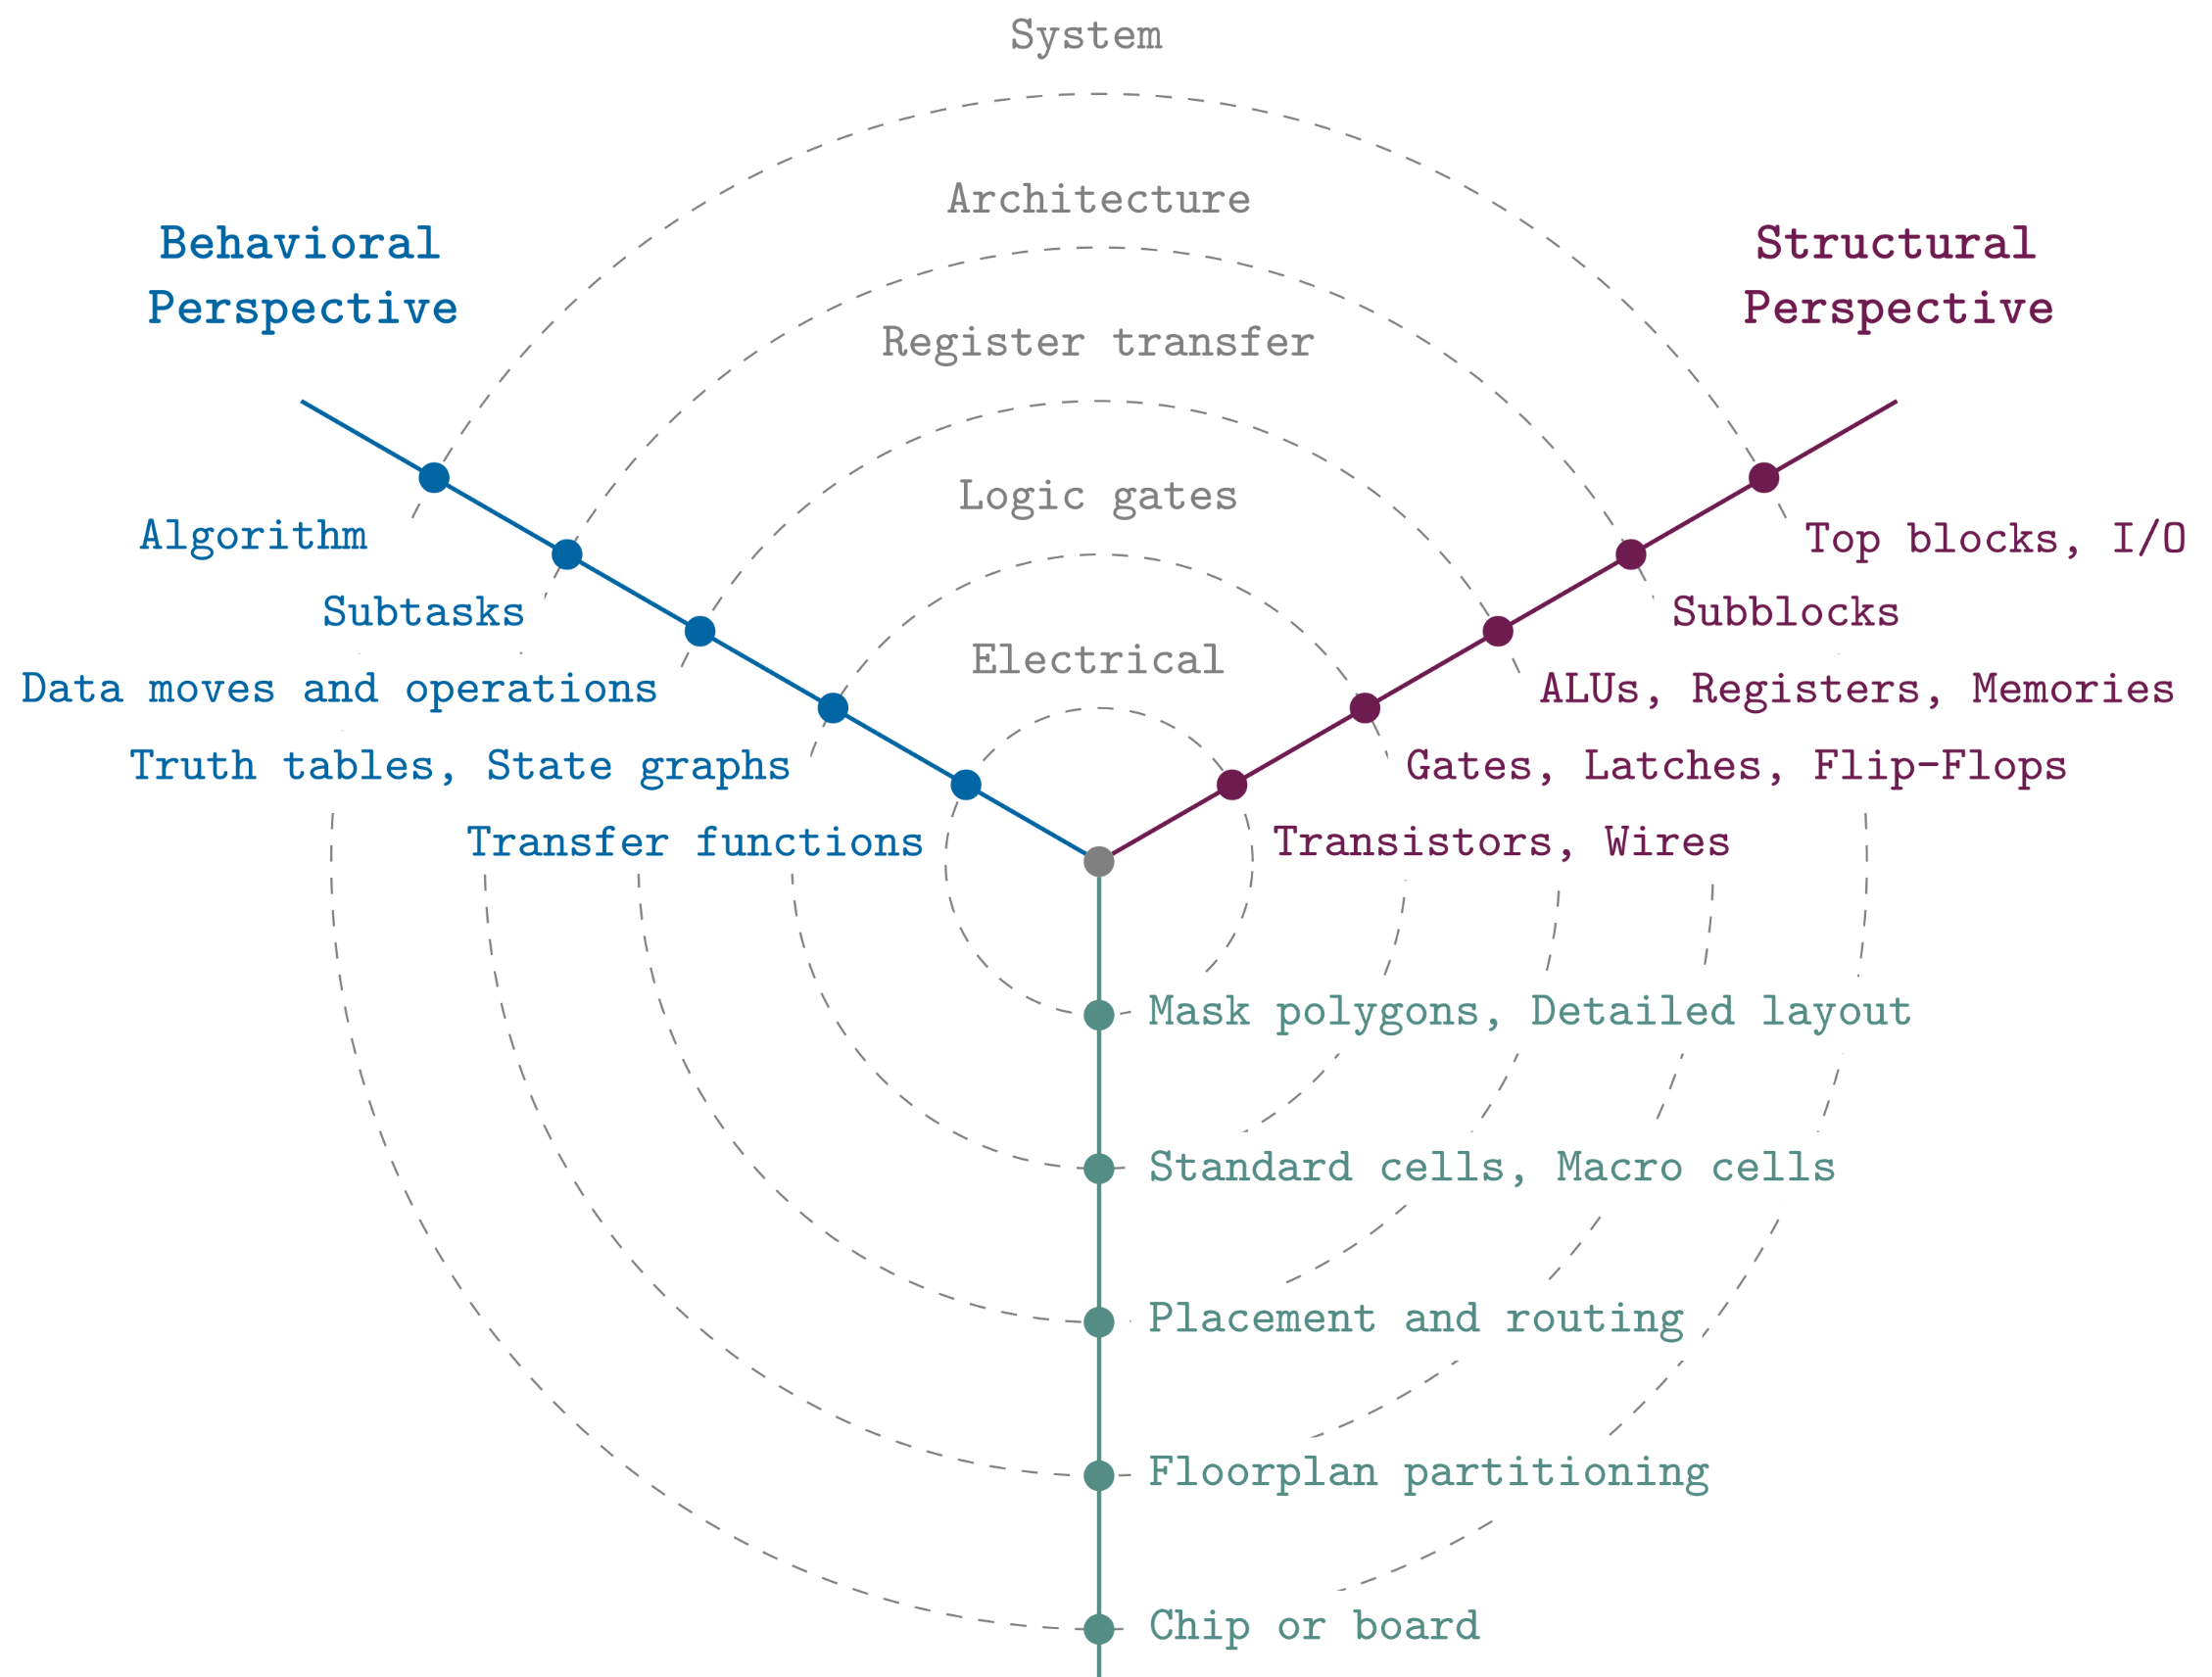
\includegraphics[width=\linewidth]{Images/DevelopmentModel.png}
        \end{minipage}%
        \hfill
        \begin{minipage}[t]{0.48\columnwidth}
            \vspace{0pt} % <-- ensures top alignment
            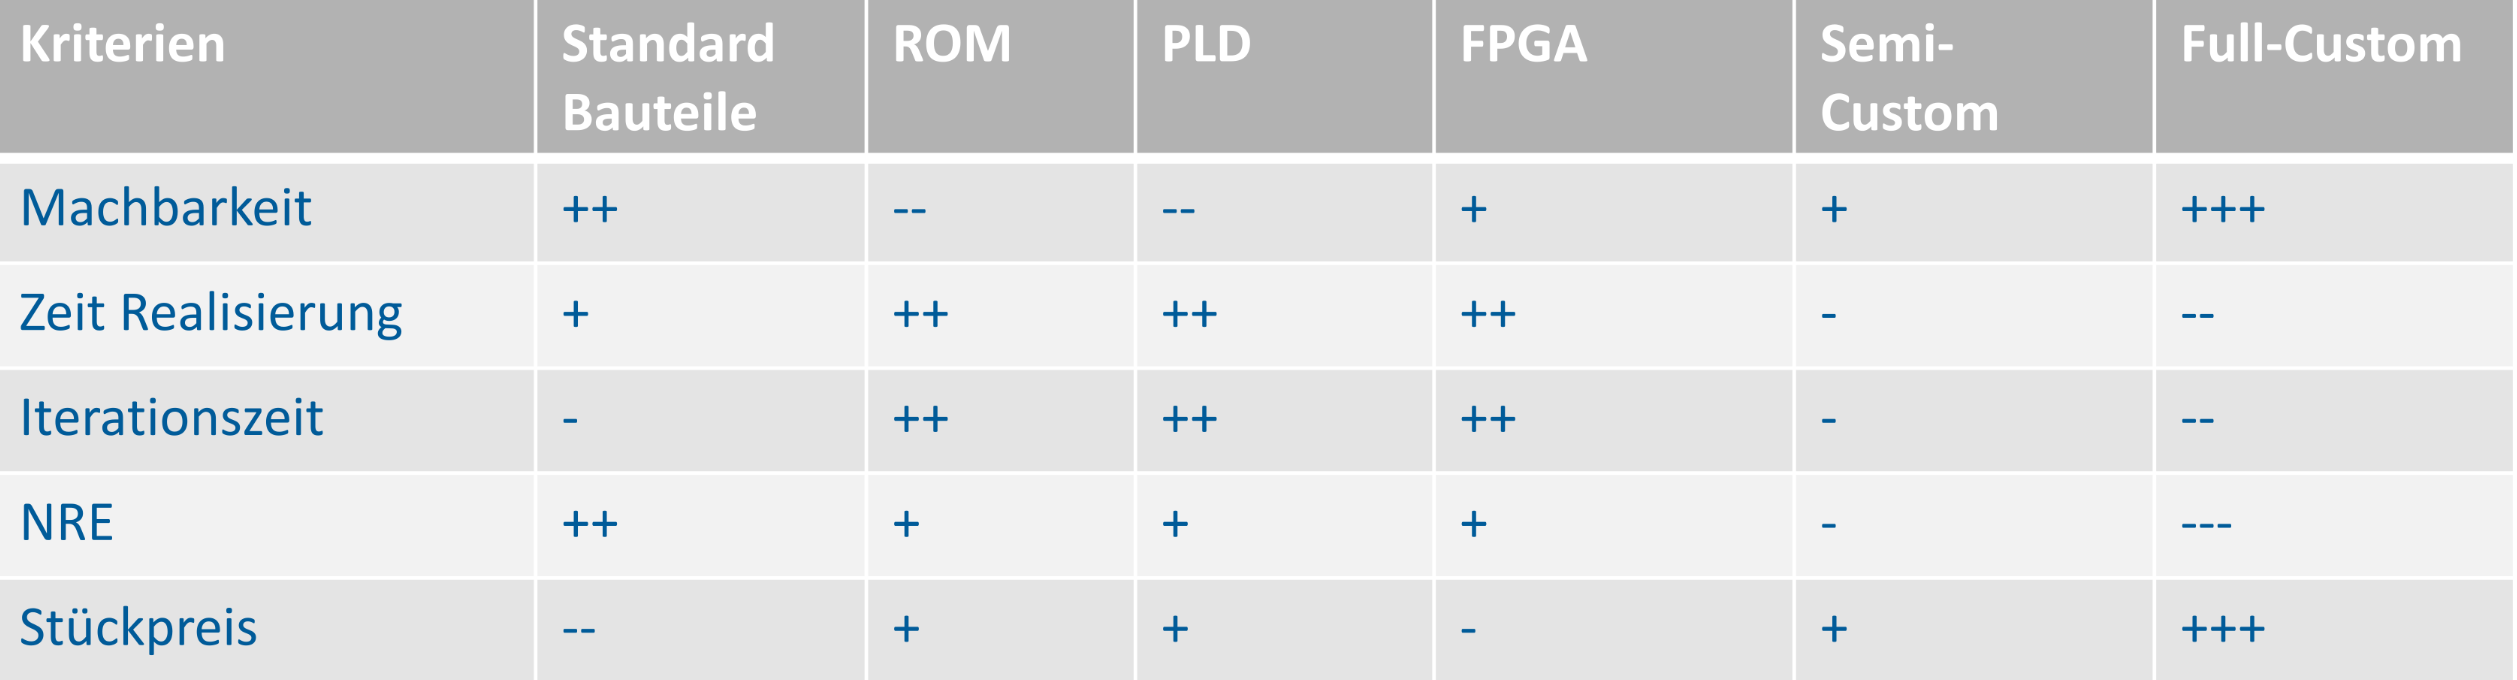
\includegraphics[width=\linewidth]{Images/WhalDerRealisirungsform.png}\\[1ex]
            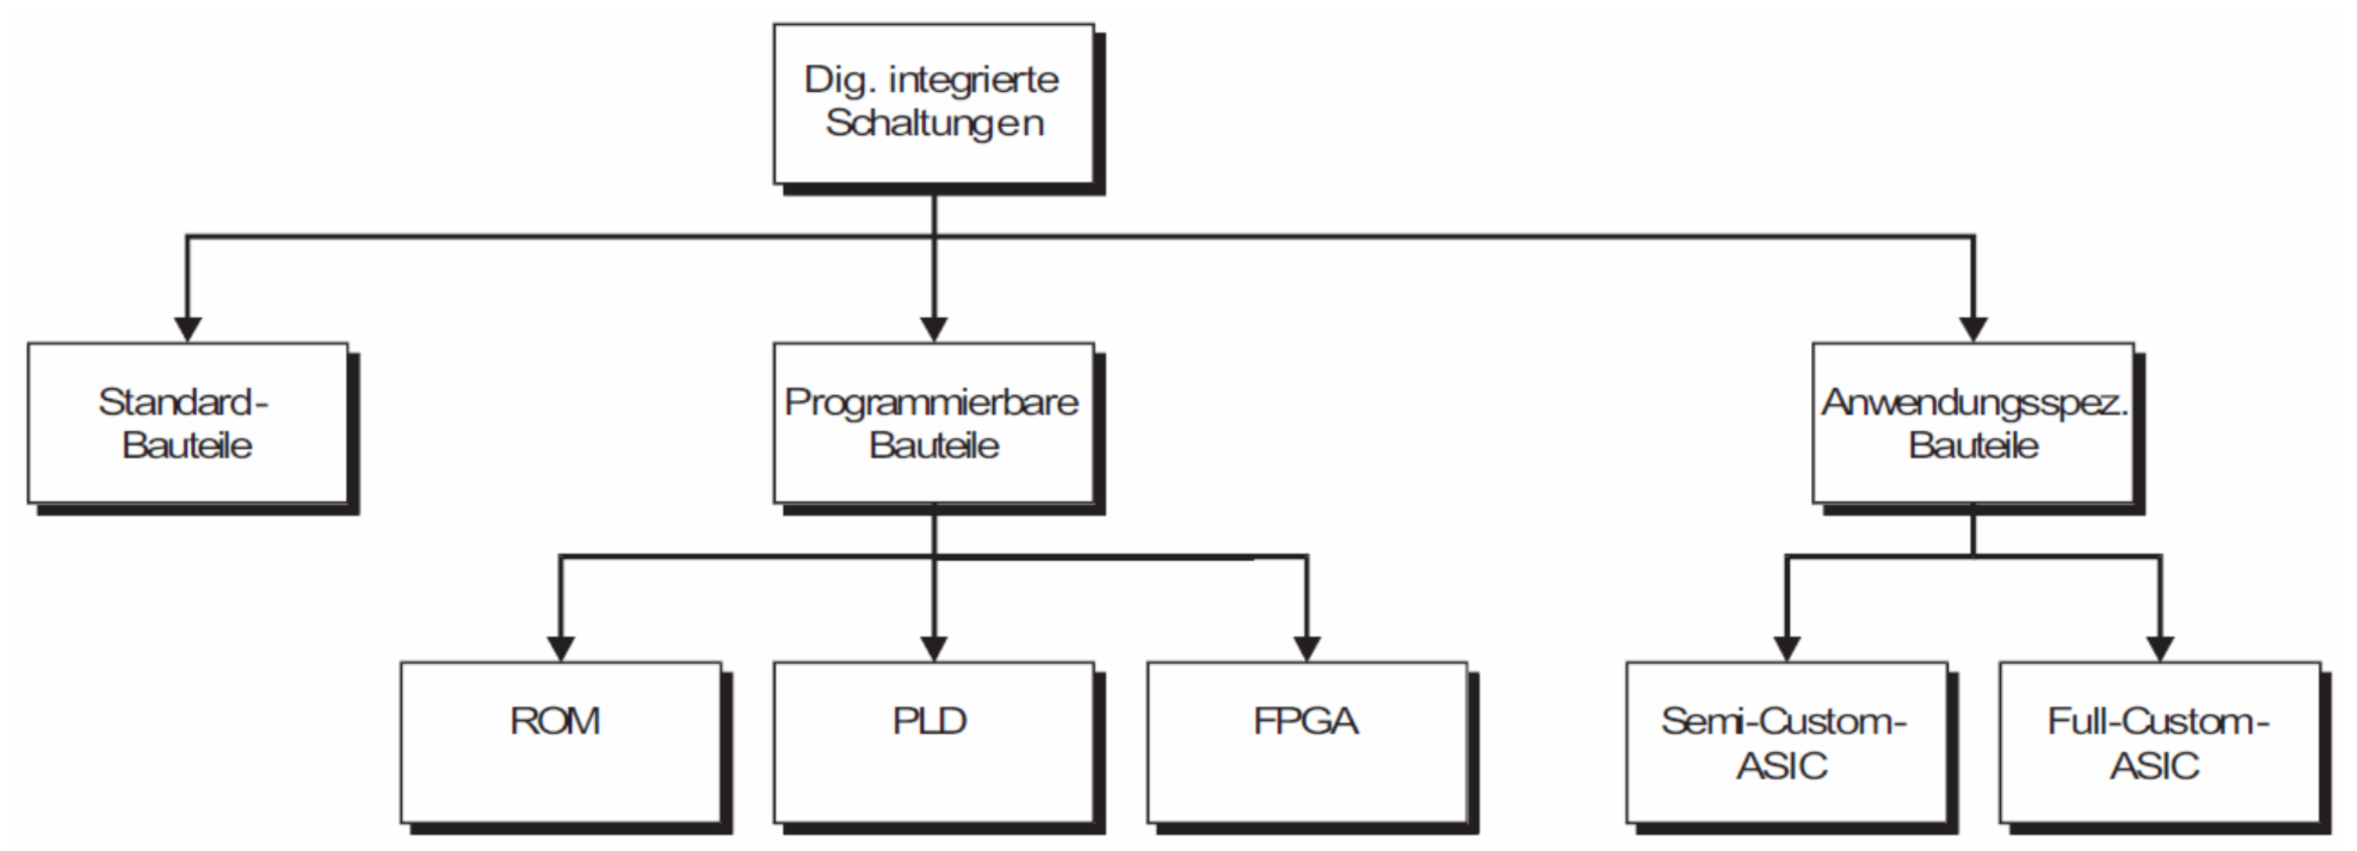
\includegraphics[width=\linewidth]{Images/ClassificationeDeiComponenti.png}
        \end{minipage}

    % \subsection{Guida al design}
    %         \begin{minipage}[t]{0.48\columnwidth}
    %             \begin{itemize}[left=0pt]
    %                 \item Design - Entry
    %                 \item Funktionale Simulation
    %                 \item Synthese
    %                 \item Implementierung
    %                     \begin{itemize}
    %                         \item Logikoptimierung
    %                         \item Platzierung
    %                         \item Verdrahtung
    %                     \end{itemize}
    %                 \item Timing Simulation
    %                 \item Statische Timing-Analyse
    %                 \item Herstellungsdatenerzeugen
    %             \end{itemize}
    %         \end{minipage}%
    %         \hfill
    %         \begin{minipage}[t]{0.48\columnwidth}
    %             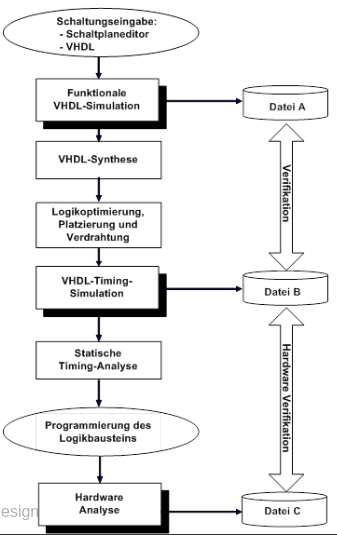
\includegraphics[width=\linewidth]{GuidaDesign.png}
    %         \end{minipage}